\input{../latex-math/basic-math}
\input{../latex-math/basic-ml}
\input{../latex-math/ml-nn}

\begin{document}

\lecturechapter{1}{Introduction}
\lecture{Introduction}
%%%%%%%%%%%%%%%%%%%%%%%%%%%%%%%%%%%%%%%%%%%%%%%%%%%%%%%%%%%%%%%%%%

\begin{frame} {What is Deep Learning}
\begin{center}
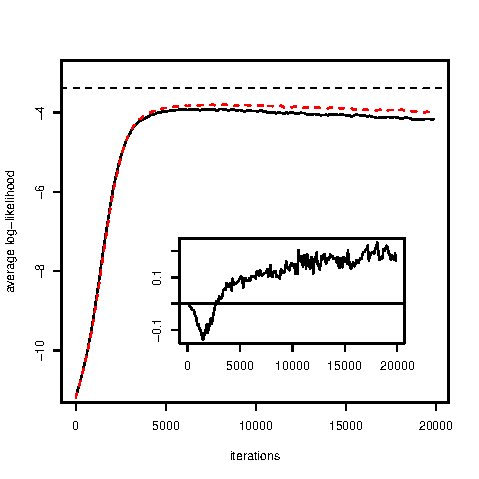
\includegraphics[width=0.95\textwidth]{../plots/learning.pdf}
\end{center}
\vspace{-.5cm}
\begin{itemize}
\item Deep learning is the use of artificial neural networks to
construct models on large amounts of (unstructured) data.
\end{itemize}
\end{frame}
%%%%%%%%%%%%%%%%%%%%%%%%%%%%%%%%%%%%%%%%%%%%%%%%%%%%%%%%%%%%%%%%%%

\begin{frame} {Deep Learning and Neural Networks}
\begin{itemize}
\item Deep learning and neural networks are mostly equivalent.
\vspace{.3cm}
\item Deep learning itself is not \textit{new}:
\begin{itemize}
\item Neural networks have been around since the 70s
\item \textit{Deep} neural networks, i.e., networks with multiple hidden layers, are not much younger.
\end{itemize}
\vspace{.3cm}
\item Why everybody is talking about deep learning now:
\begin{enumerate}
\vspace{.1cm}
\item Specialized, powerful hardware allows training of huge neural networks to push the state-of-the-art on difficult problems.
\vspace{.2cm}
\item Large amount of data is available.
\vspace{.2cm}
\item Special network architectures for image/text data.
\vspace{.2cm}
\item Better optimization and regularization strategies.
\end{enumerate}
\end{itemize}
\end{frame}
%%%%%%%%%%%%%%%%%%%%%%%%%%%%%%%%%%%%%%%%%%%%%%%%%%%%%%%%%%%%%%%%%%

\begin{frame}{Image Classification with Neural Networks}
\begin{aquote}{Y. Bengio}
Machine learning algorithms, inspired by the brain, based on learning multiple levels of representation/abstraction.   
\end{aquote}
\begin{overlayarea}{\textwidth}{\textheight}
\centering
\only<1>{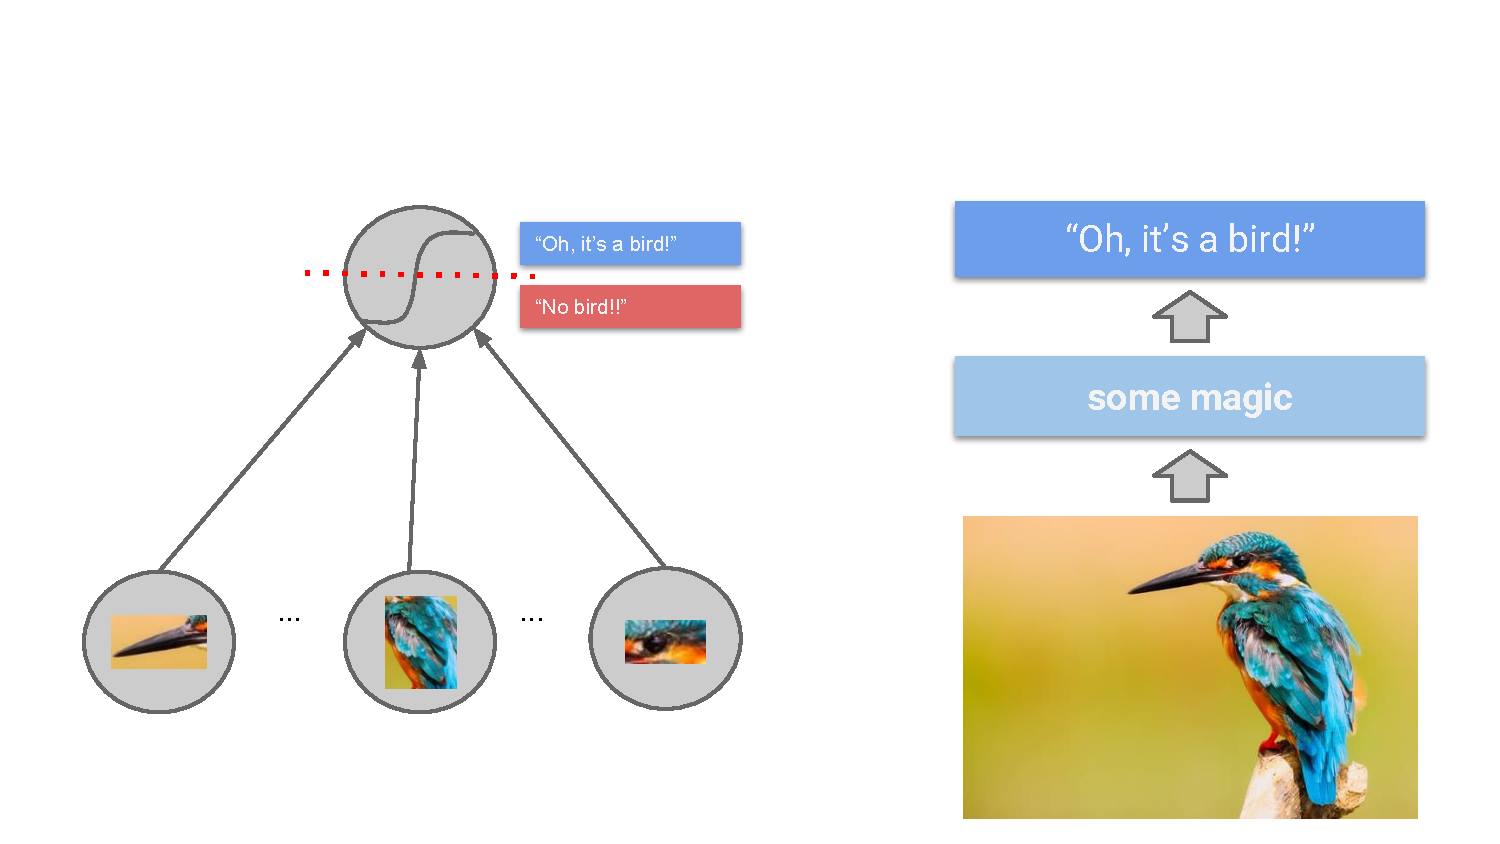
\includegraphics[width=0.7\textwidth]{../plots/bird1.pdf}}
\only<1>{\\ \footnotesize{Caption 1}}
\only<2>{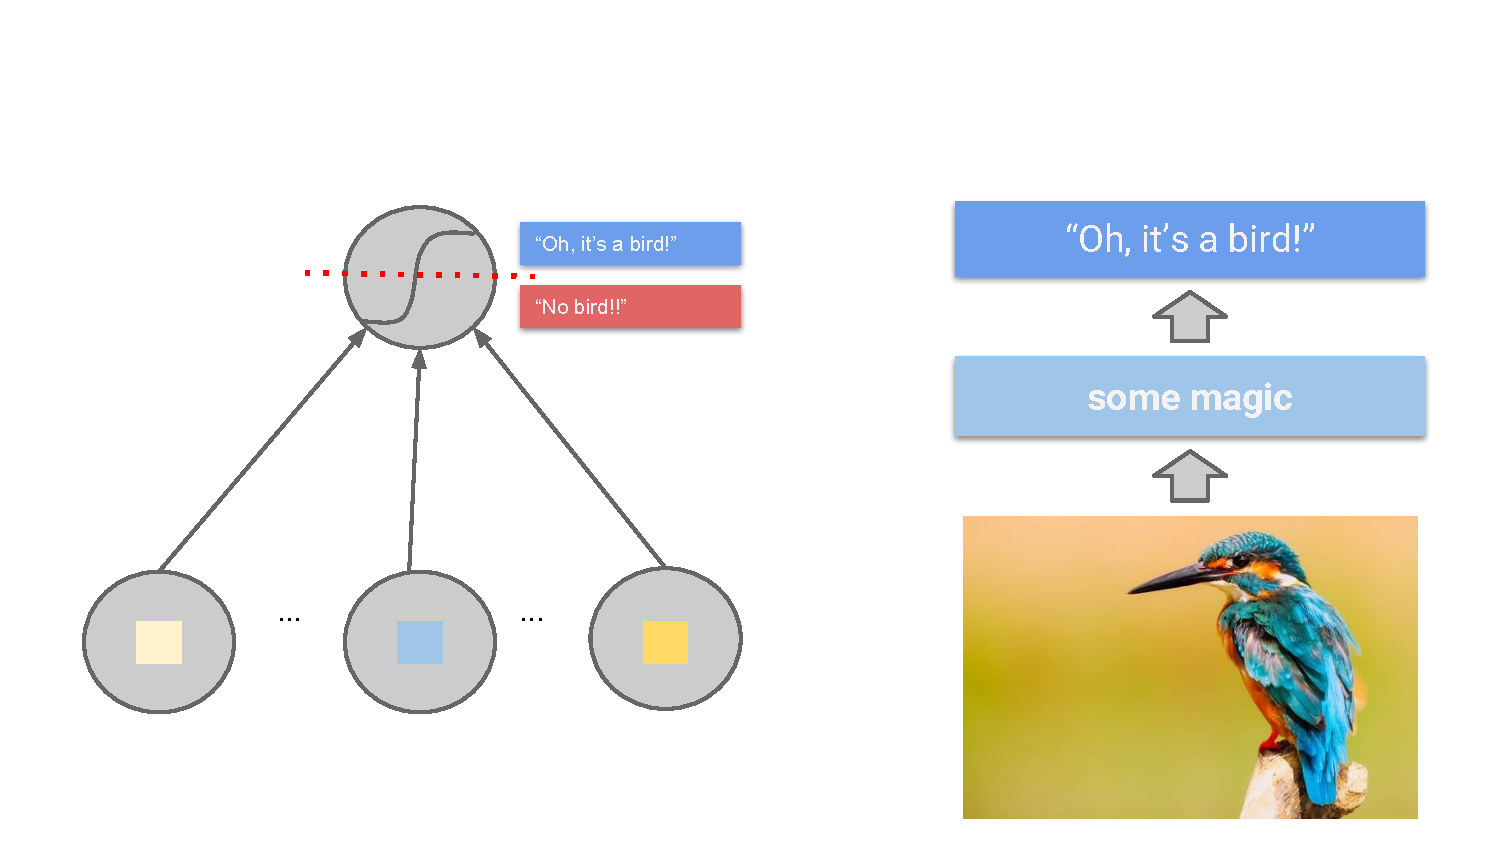
\includegraphics[width=0.7\textwidth]{../plots/bird2.pdf}}
\only<2>{\\ \footnotesize{Caption 2}}
\only<3>{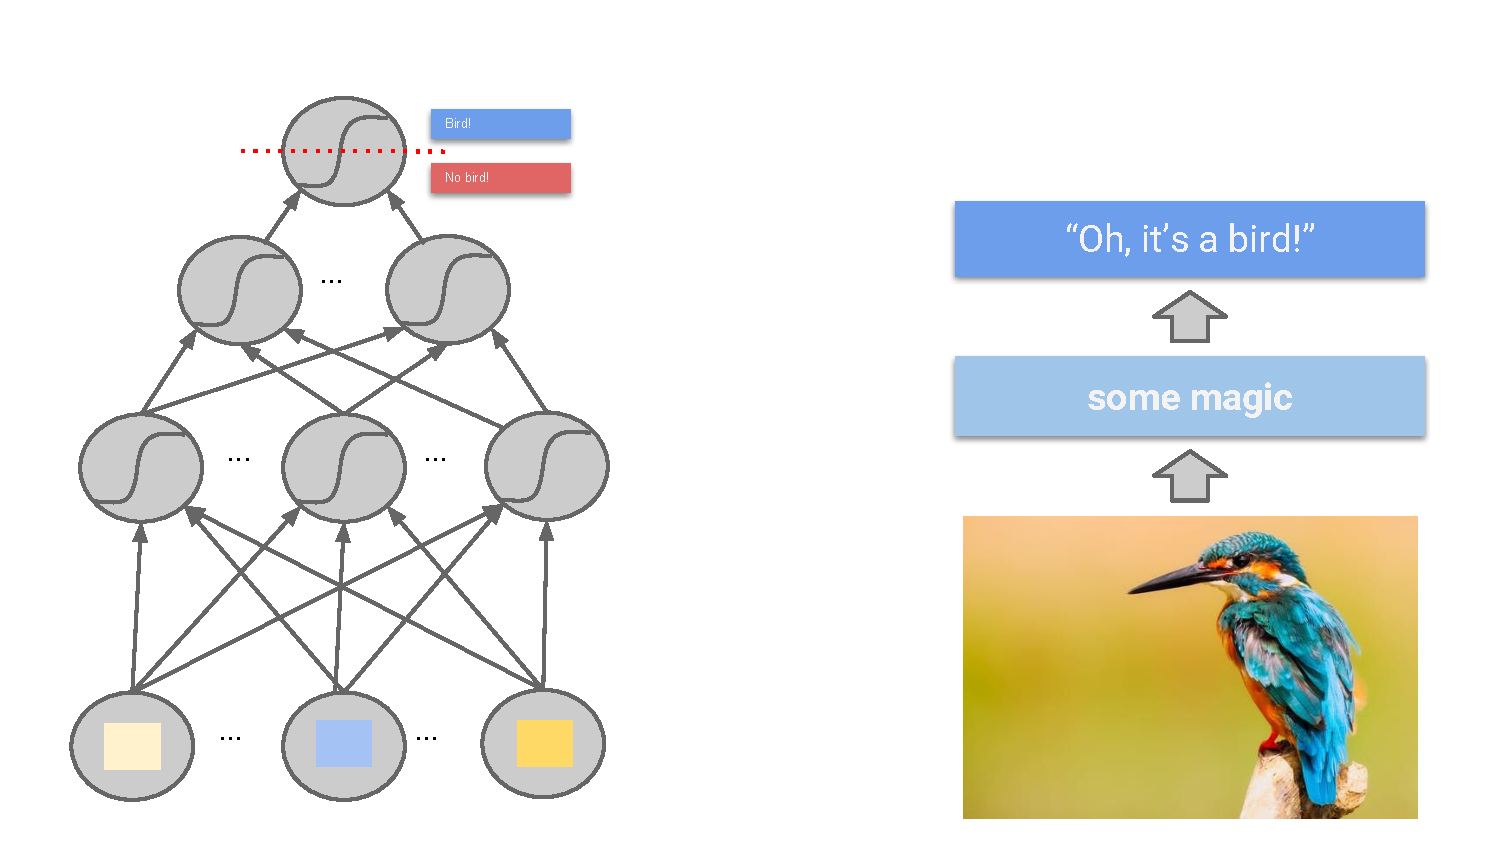
\includegraphics[width=0.7\textwidth]{../plots/bird3.pdf}}
\only<3>{\\ \footnotesize{Caption 3}}
\only<4>{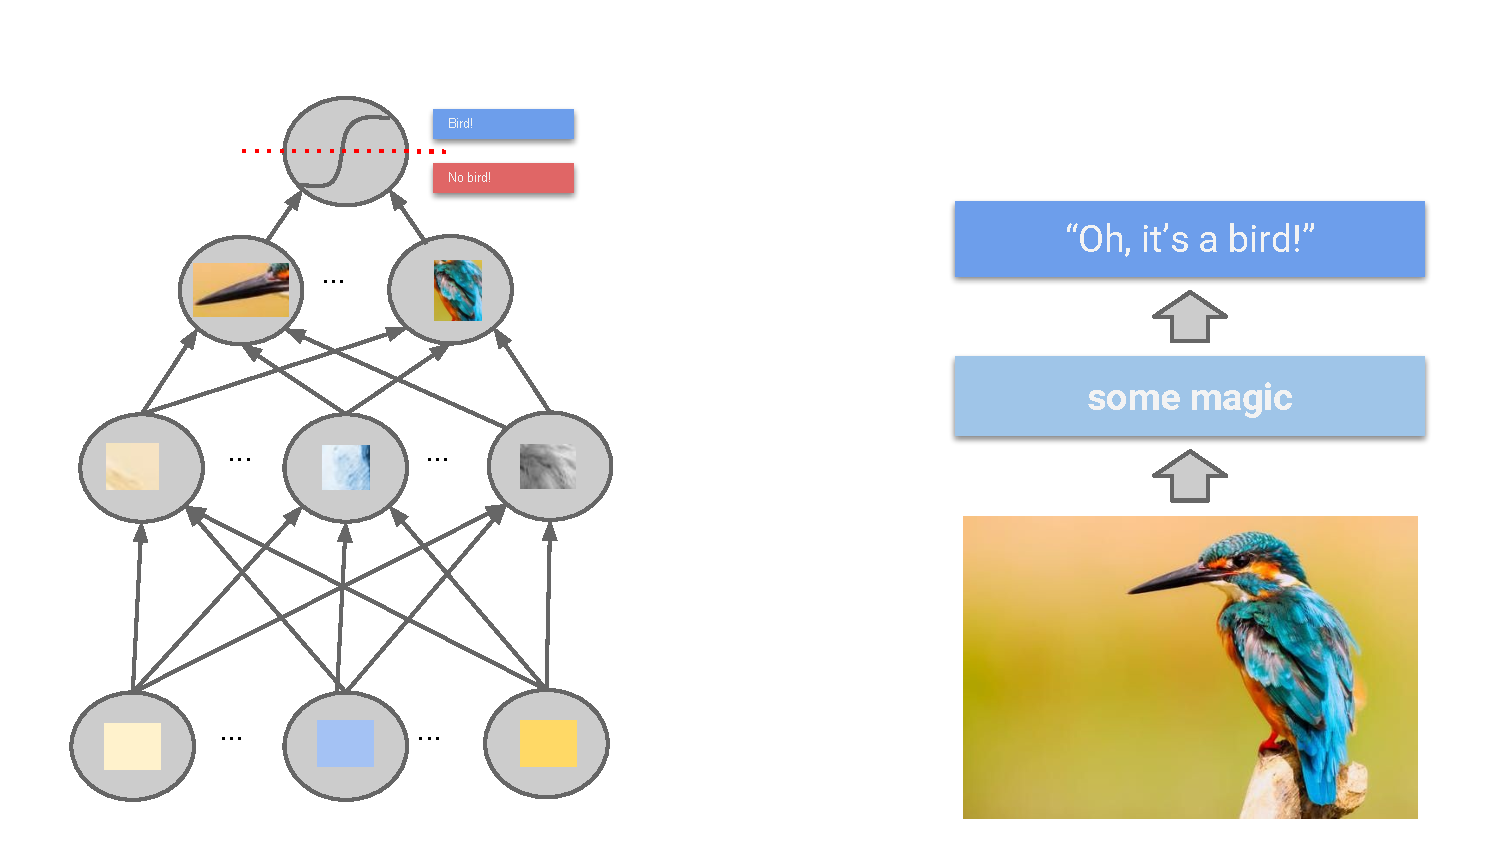
\includegraphics[width=0.7\textwidth]{../plots/bird4.pdf}}
\only<4>{\\ \footnotesize{Caption 4}}
\end{overlayarea}
\end{frame}
%%%%%%%%%%%%%%%%%%%%%%%%%%%%%%%%%%%%%%%%%%%%%%%%%%%%%%%%%%%%%%%%%%

\begin{frame} {Possible use-cases}
\textbf{Deep learning can be extremely valuable if the data has these properties:}
\vspace{.2cm}
\begin{itemize}
\item It is high dimensional.
\item Each single feature itself is not very informative but only a combination of them might be.
\item There is a large amount of training data.
\end{itemize}
\vspace{.7cm}
\textbf{This implies that for tabular data, deep learning is almost never the correct model choice.}
\vspace{.2cm}
\begin{itemize}
\item Models like random forests or gradient boosting will outperform deep learning most of the time.
\item One exception is data with categorical features with many levels.
\end{itemize}

\end{frame}
%%%%%%%%%%%%%%%%%%%%%%%%%%%%%%%%%%%%%%%%%%%%%%%%%%%%%%%%%%%%%%%%%%

\begin{frame} {Possible use-case: Images}
\begin{itemize}
\item \textbf{High Dimensional}: A color image with $255 \times 255$ (3 Colors) pixels already has $195075$ features.
\vspace{.1cm}
\item \textbf{Informative}: A single pixel is not meaningful in itself.
\vspace{.1cm}
\item \textbf{Training Data}: Depending on applications huge amounts of data are available.
\end{itemize}
\vspace{.3cm}
Architecture: \textbf{C}onvolutional \textbf{N}eural \textbf{N}etworks (CNN)
\begin{figure}
\centering
\scalebox{.85}{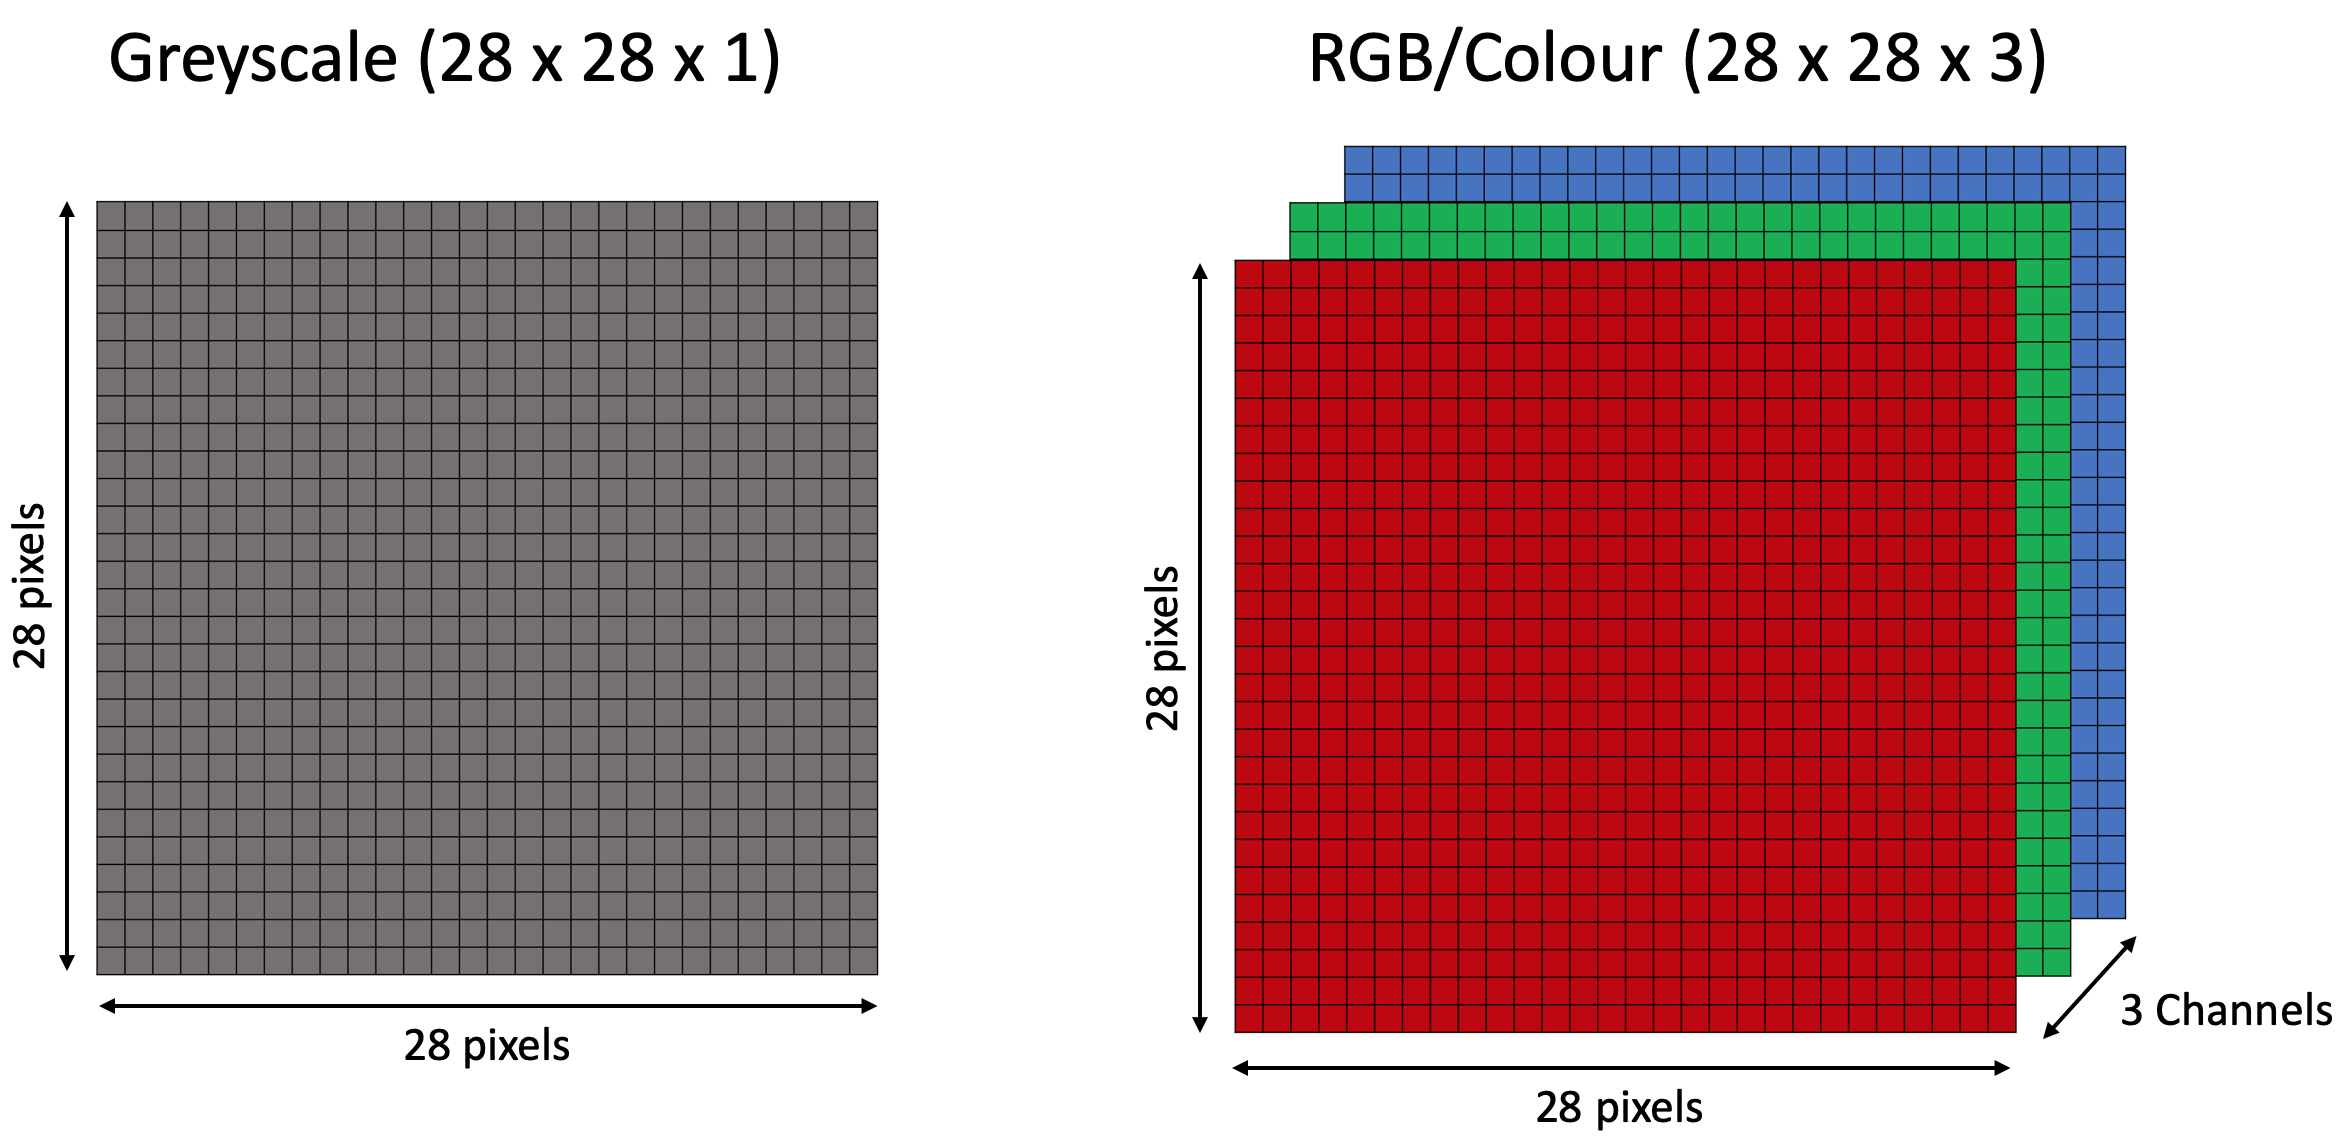
\includegraphics{../plots/three_channels.png}}
\\
\tiny{Credit: https://medium.com/@RaghavPrabhu/understanding-of-convolutional-neural-network-cnn-deep-learning-99760835f148}
\end{figure}
%https://medium.com/@RaghavPrabhu/understanding-of-convolutional-neural-network-cnn-deep-learning-99760835f148
\end{frame}
%%%%%%%%%%%%%%%%%%%%%%%%%%%%%%%%%%%%%%%%%%%%%%%%%%%%%%%%%%%%%%%%%%

\begin{frame} {Possible use-case: Images}
\begin{figure}
\centering
\scalebox{.7}{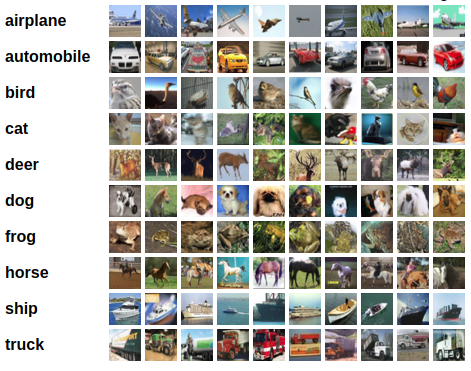
\includegraphics{../plots/classification.png}}
\\
\tiny{Credit: Alex Krizhevsky (2009)}
\end{figure}
\textbf{Image classification} tries to predict a single label for each image.
\footnotesize CIFAR-10 is a well-known dataset used for image classification. It consists of $60,000$ $32x32$ color images containing one of $10$ object classes, with $6000$ images per class. 
\end{frame}
%%%%%%%%%%%%%%%%%%%%%%%%%%%%%%%%%%%%%%%%%%%%%%%%%%%%%%%%%%%%%%%%%%

\begin{frame} {Possible use-case: Images}
\begin{figure}
\centering
\scalebox{0.8}{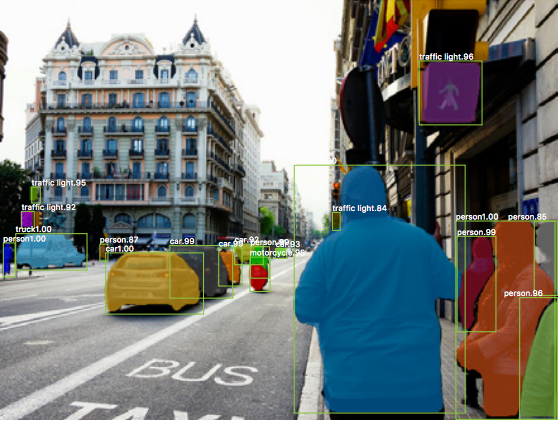
\includegraphics{../plots/maskrcnn.png}}
\\
\tiny{Credit: Kaiming He (2017)}
\end{figure}
\textbf{Object Detection}
\footnotesize Mask R-CNN is a general framework for instance segmentation, which efficiently detects objects in an image while simultaneously generating a high-quality segmentation mask for each instance.
\end{frame}
%%%%%%%%%%%%%%%%%%%%%%%%%%%%%%%%%%%%%%%%%%%%%%%%%%%%%%%%%%%%%%%%%%

\begin{frame} {Possible use-case: Images}
\begin{figure}
\centering
\scalebox{.8}{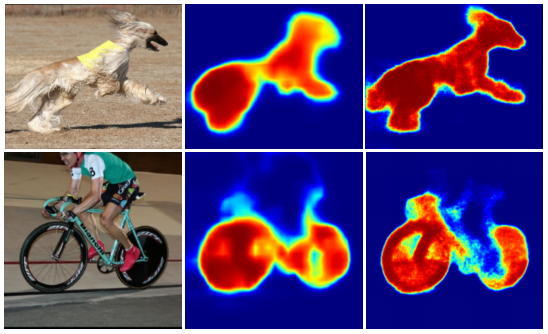
\includegraphics{../plots/segmentation.png}}
\\
\tiny{Credit: Hyeonwoo Noh (2015)} 
\end{figure}
\textbf{Image segmentation} partitions the image into (multiple) segments.
\end{frame}
%%%%%%%%%%%%%%%%%%%%%%%%%%%%%%%%%%%%%%%%%%%%%%%%%%%%%%%%%%%%%%%%%%

\begin{frame} {Possible use-case: Text}
\begin{itemize}
\item \textbf{High Dimensional}: Each word can be a single feature (~300000 words in the German language).
\vspace{.1cm}
\item \textbf{Informative}: A single word does not provide much context.
\vspace{.1cm}
\item \textbf{Training Data}: Huge amounts of text data available.
\end{itemize}
\vspace{.3cm}
Architecture: \textbf{R}ecurrent \textbf{N}eural \textbf{N}etworks (RNN)
\begin{figure}
\centering
\scalebox{.75}{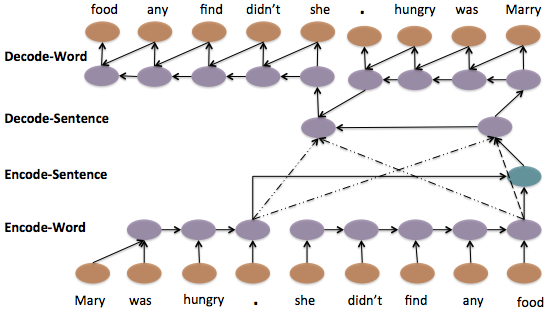
\includegraphics{../plots/hierarchical_sequence.png}}
\\
\tiny{Credit: Li, Luong, and Jurafsky (2015)} 
%https://arxiv.org/abs/1506.01057
\end{figure}
\end{frame}
%%%%%%%%%%%%%%%%%%%%%%%%%%%%%%%%%%%%%%%%%%%%%%%%%%%%%%%%%%%%%%%%%%

\begin{frame} {Possible use-case: Text}
Applications:
\vspace{.7cm}
\begin{itemize}
\item \textbf{N}atural \textbf{L}anguage \textbf{P}rocessing, e.g.,
\begin{itemize}
\item Sentiment Analysis
\vspace{.3cm}
\item Email Classification
\vspace{.3cm}
\item Chat-bots
\vspace{.3cm}
\item $...$
\end{itemize}
\vspace{.7cm}
\item Modeling Sequential Data (Time-Series, Speech)
\end{itemize}
\end{frame}
%%%%%%%%%%%%%%%%%%%%%%%%%%%%%%%%%%%%%%%%%%%%%%%%%%%%%%%%%%%%%%%%%%

\begin{frame} {Possible use-case: Text}
\begin{figure}
\centering
\scalebox{.9}{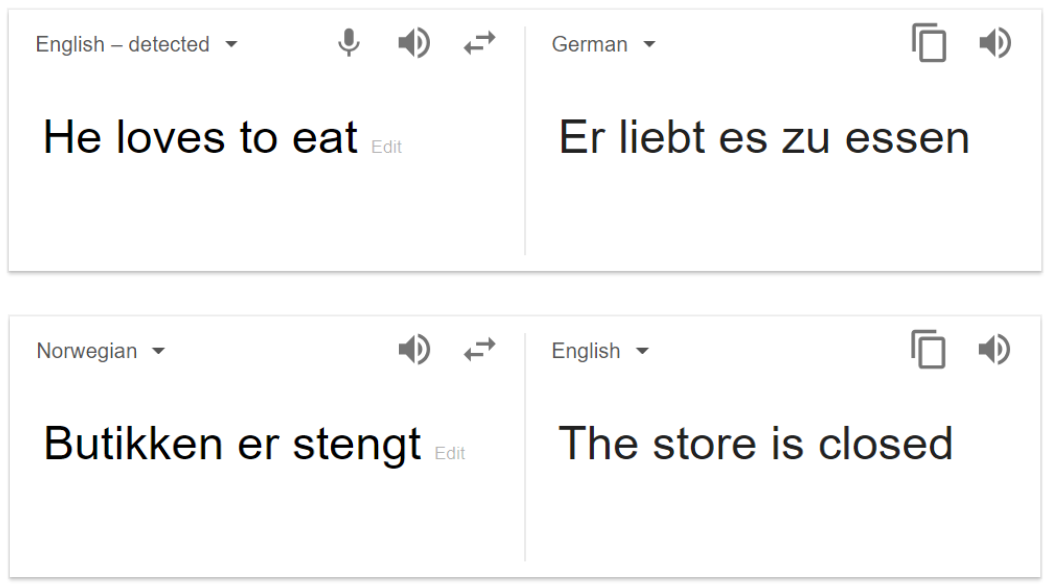
\includegraphics{../plots/nmt.png}}
\end{figure}
\textbf{Machine Translation} (e.g. google translate) 
Neural machine translation exploits neural networks to predict the likelihood of a sequence of words, typically modeling entire sentences in a single integrated model.
\end{frame}
%%%%%%%%%%%%%%%%%%%%%%%%%%%%%%%%%%%%%%%%%%%%%%%%%%%%%%%%%%%%%%%%%%

\begin{frame} {Applications of Deep Learning: Speech}
\begin{figure}
\centering
\scalebox{.9}{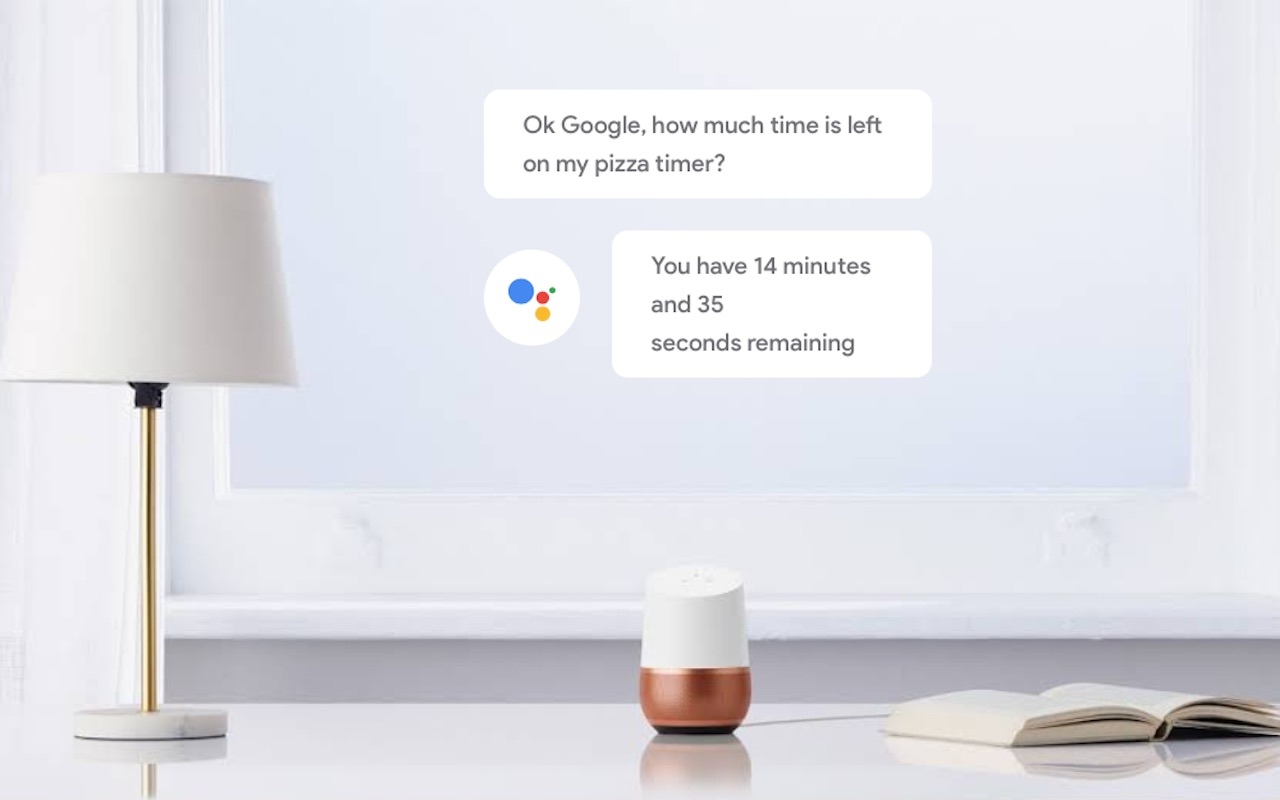
\includegraphics{../plots/speech_goog.jpg}}
\end{figure}
\textbf{Speech Recognition and Generation} (e.g. google assistant)
Neural network extracts features from audio data in order to classify emotions in speech.
\end{frame}
%%%%%%%%%%%%%%%%%%%%%%%%%%%%%%%%%%%%%%%%%%%%%%%%%%%%%%%%%%%%%%%%%%

\endlecture
\end{document}